\documentclass[a4paper]{book}
\usepackage[margin=1in]{geometry}
\usepackage[T1]{fontenc}
\usepackage[utf8]{inputenc}
\usepackage[hidelinks]{hyperref}
\usepackage{amsmath}
\usepackage{amssymb}
\usepackage{enumerate}
\usepackage{setspace}
\usepackage{listings}
\usepackage{xcolor}
\usepackage{amsthm}
\usepackage{xspace}
\usepackage{adjustbox}
\usepackage{booktabs} 
\usepackage{array}    
\usepackage{adjustbox} 
\usepackage{colortbl}
\usepackage{graphicx}

% Configuration pour les listings de code
\definecolor{codebg}{RGB}{245,245,245}
\lstset{
    backgroundcolor=\color{codebg},
    basicstyle=\ttfamily\small,
    frame=single,
    breaklines=true,
    columns=fullflexible,
    keywordstyle=\color{blue},
    commentstyle=\color{gray},
    stringstyle=\color{orange},
    showstringspaces=false
}
\setstretch{1.15}

%----- TITLE PAGE INFO -----%

\title{\Huge \textbf{Multilayer Switch (MLS) Workbook}\\
       \Large VLANs, Inter-VLAN Routing, and Troubleshooting}
\author{\Large Written for Networking Students and Professionals}
\date{\today}

\begin{document}

%----- MODERN TITLE PAGE -----%

\begin{titlepage}
    \centering

    \vspace*{4cm}
    {\Huge \textbf{Multilayer Switch (MLS) Workbook}\par}
    \vspace{0.8cm}
    {\Large A Hands-On Guide to VLAN Configuration, Inter-VLAN Routing, and Troubleshooting\par}
    \vspace{0.3cm}
    \rule{0.9\textwidth}{1pt}
    
    \vspace{0.6cm}
    {\large \textbf{Mehdi JAFARI ZADEH}}\par
    \vspace{0.3cm}

    \vfill
    \textbf{Date:} \today
    \vspace{2cm}
\end{titlepage}

\tableofcontents
\newpage

\chapter{Tutorial: Inter-VLAN Routing with ROAS and Multilayer Switches}
\section{Introduction}
Virtual Local Area Networks (VLANs) are used in network environments to segment traffic and improve performance and security. However, devices in separate VLANs cannot communicate with each other by default. Inter-VLAN routing allows devices from different VLANs to communicate, and this can be achieved through two main methods: \textbf{Router-on-a-Stick (ROAS)} and \textbf{Multilayer Switch (MLS) Inter-VLAN Routing}.

\section{Router-on-a-Stick (ROAS)}
\subsection{Overview}
Router-on-a-Stick (ROAS) is a method of inter-VLAN routing that uses a single router with a trunk link to a switch. The router performs all routing functions between VLANs.

\subsection{How It Works}
\begin{enumerate}
    \item A trunk link is established between the router and the switch.
    \item Subinterfaces are created on the router for each VLAN.
    \item Each subinterface is assigned an IP address that acts as the default gateway for its respective VLAN.
    \item The switch forwards VLAN-tagged traffic to the router, which then routes it to the appropriate VLAN.
\end{enumerate}

\subsection{Configuration Steps}
\subsubsection{On the Switch}
\begin{lstlisting}
configure terminal
interface GigabitEthernet0/1
switchport mode trunk
switchport trunk allowed vlan 10,20
exit
\end{lstlisting}

\subsubsection{On the Router}
\begin{lstlisting}
configure terminal
interface GigabitEthernet0/1
no shutdown
interface GigabitEthernet0/1.10
encapsulation dot1Q 10
ip address 192.168.10.1 255.255.255.0
exit
interface GigabitEthernet0/1.20
encapsulation dot1Q 20
ip address 192.168.20.1 255.255.255.0
exit
\end{lstlisting}

\subsection{Advantages and Disadvantages}
\textbf{Advantages:}
\begin{itemize}
    \item Cost-effective for small networks.
    \item Simple to implement.
\end{itemize}

\textbf{Disadvantages:}
\begin{itemize}
    \item Limited scalability due to reliance on a single router interface.
    \item Potential bottleneck due to the router processing all inter-VLAN traffic.
\end{itemize}

\section{Inter-VLAN Routing with a Multilayer Switch (MLS)}
\subsection{Overview}
A multilayer switch (MLS) can perform routing functions at Layer 3, eliminating the need for an external router.

\subsection{How It Works}
\begin{enumerate}
    \item The MLS is configured with Switched Virtual Interfaces (SVIs) for each VLAN.
    \item Each SVI is assigned an IP address that acts as the default gateway for its VLAN.
    \item The MLS handles inter-VLAN routing internally, reducing latency.
\end{enumerate}

\subsection{Configuration Steps}
\subsubsection{Enable Routing on the Switch}
\begin{lstlisting}
configure terminal
ip routing
\end{lstlisting}

\subsubsection{Create and Configure SVIs}
\begin{lstlisting}
interface vlan 10
ip address 192.168.10.1 255.255.255.0
no shutdown
exit
interface vlan 20
ip address 192.168.20.1 255.255.255.0
no shutdown
exit
\end{lstlisting}

\subsection{Advantages and Disadvantages}
\textbf{Advantages:}
\begin{itemize}
    \item Higher performance as traffic remains within the switch.
    \item Scalability for larger networks.
    \item Reduced latency due to elimination of external routing hops.
\end{itemize}

\textbf{Disadvantages:}
\begin{itemize}
    \item Higher cost compared to ROAS.
    \item Requires a switch with Layer 3 capabilities.
\end{itemize}

\section{Choosing Between ROAS and MLS}
\begin{table}[h]
    \centering
    \begin{tabular}{lcc}
        \toprule
        Feature & Router-on-a-Stick (ROAS) & Multilayer Switch (MLS) \\
        \midrule
        Cost & Lower & Higher \\
        Performance & Slower (bottlenecks) & Faster \\
        Scalability & Limited & Scalable \\
        Complexity & Simple & Moderate \\
        Hardware Needed & Router \& L2 Switch & L3 Switch \\
        \bottomrule
    \end{tabular}
    \caption{Comparison of ROAS and MLS}
    \label{tab:comparison}
\end{table}

For small networks with limited VLANs, ROAS is a cost-effective solution. For larger enterprise networks requiring higher performance, MLS is the preferred method.

\section{Conclusion}
Inter-VLAN routing is essential for modern networks to ensure seamless communication between VLANs. While ROAS is a simple and cost-effective solution, MLS offers improved performance and scalability. Choosing the right method depends on network size, traffic load, and budget considerations. Implementing the correct inter-VLAN routing solution ensures an efficient, high-performing, and well-segmented network infrastructure.

\part{Exercises and Hands-On Practice}

\chapter{Network Topology for Router-on-a-Stick (ROAS)}

\section{Network Topology}
The topology below represents a \textbf{Router-on-a-Stick (ROAS) network}, where a \textbf{single router} is responsible for \textbf{inter-VLAN routing} using \textbf{subinterfaces}.

\begin{figure}[h]
    \centering
    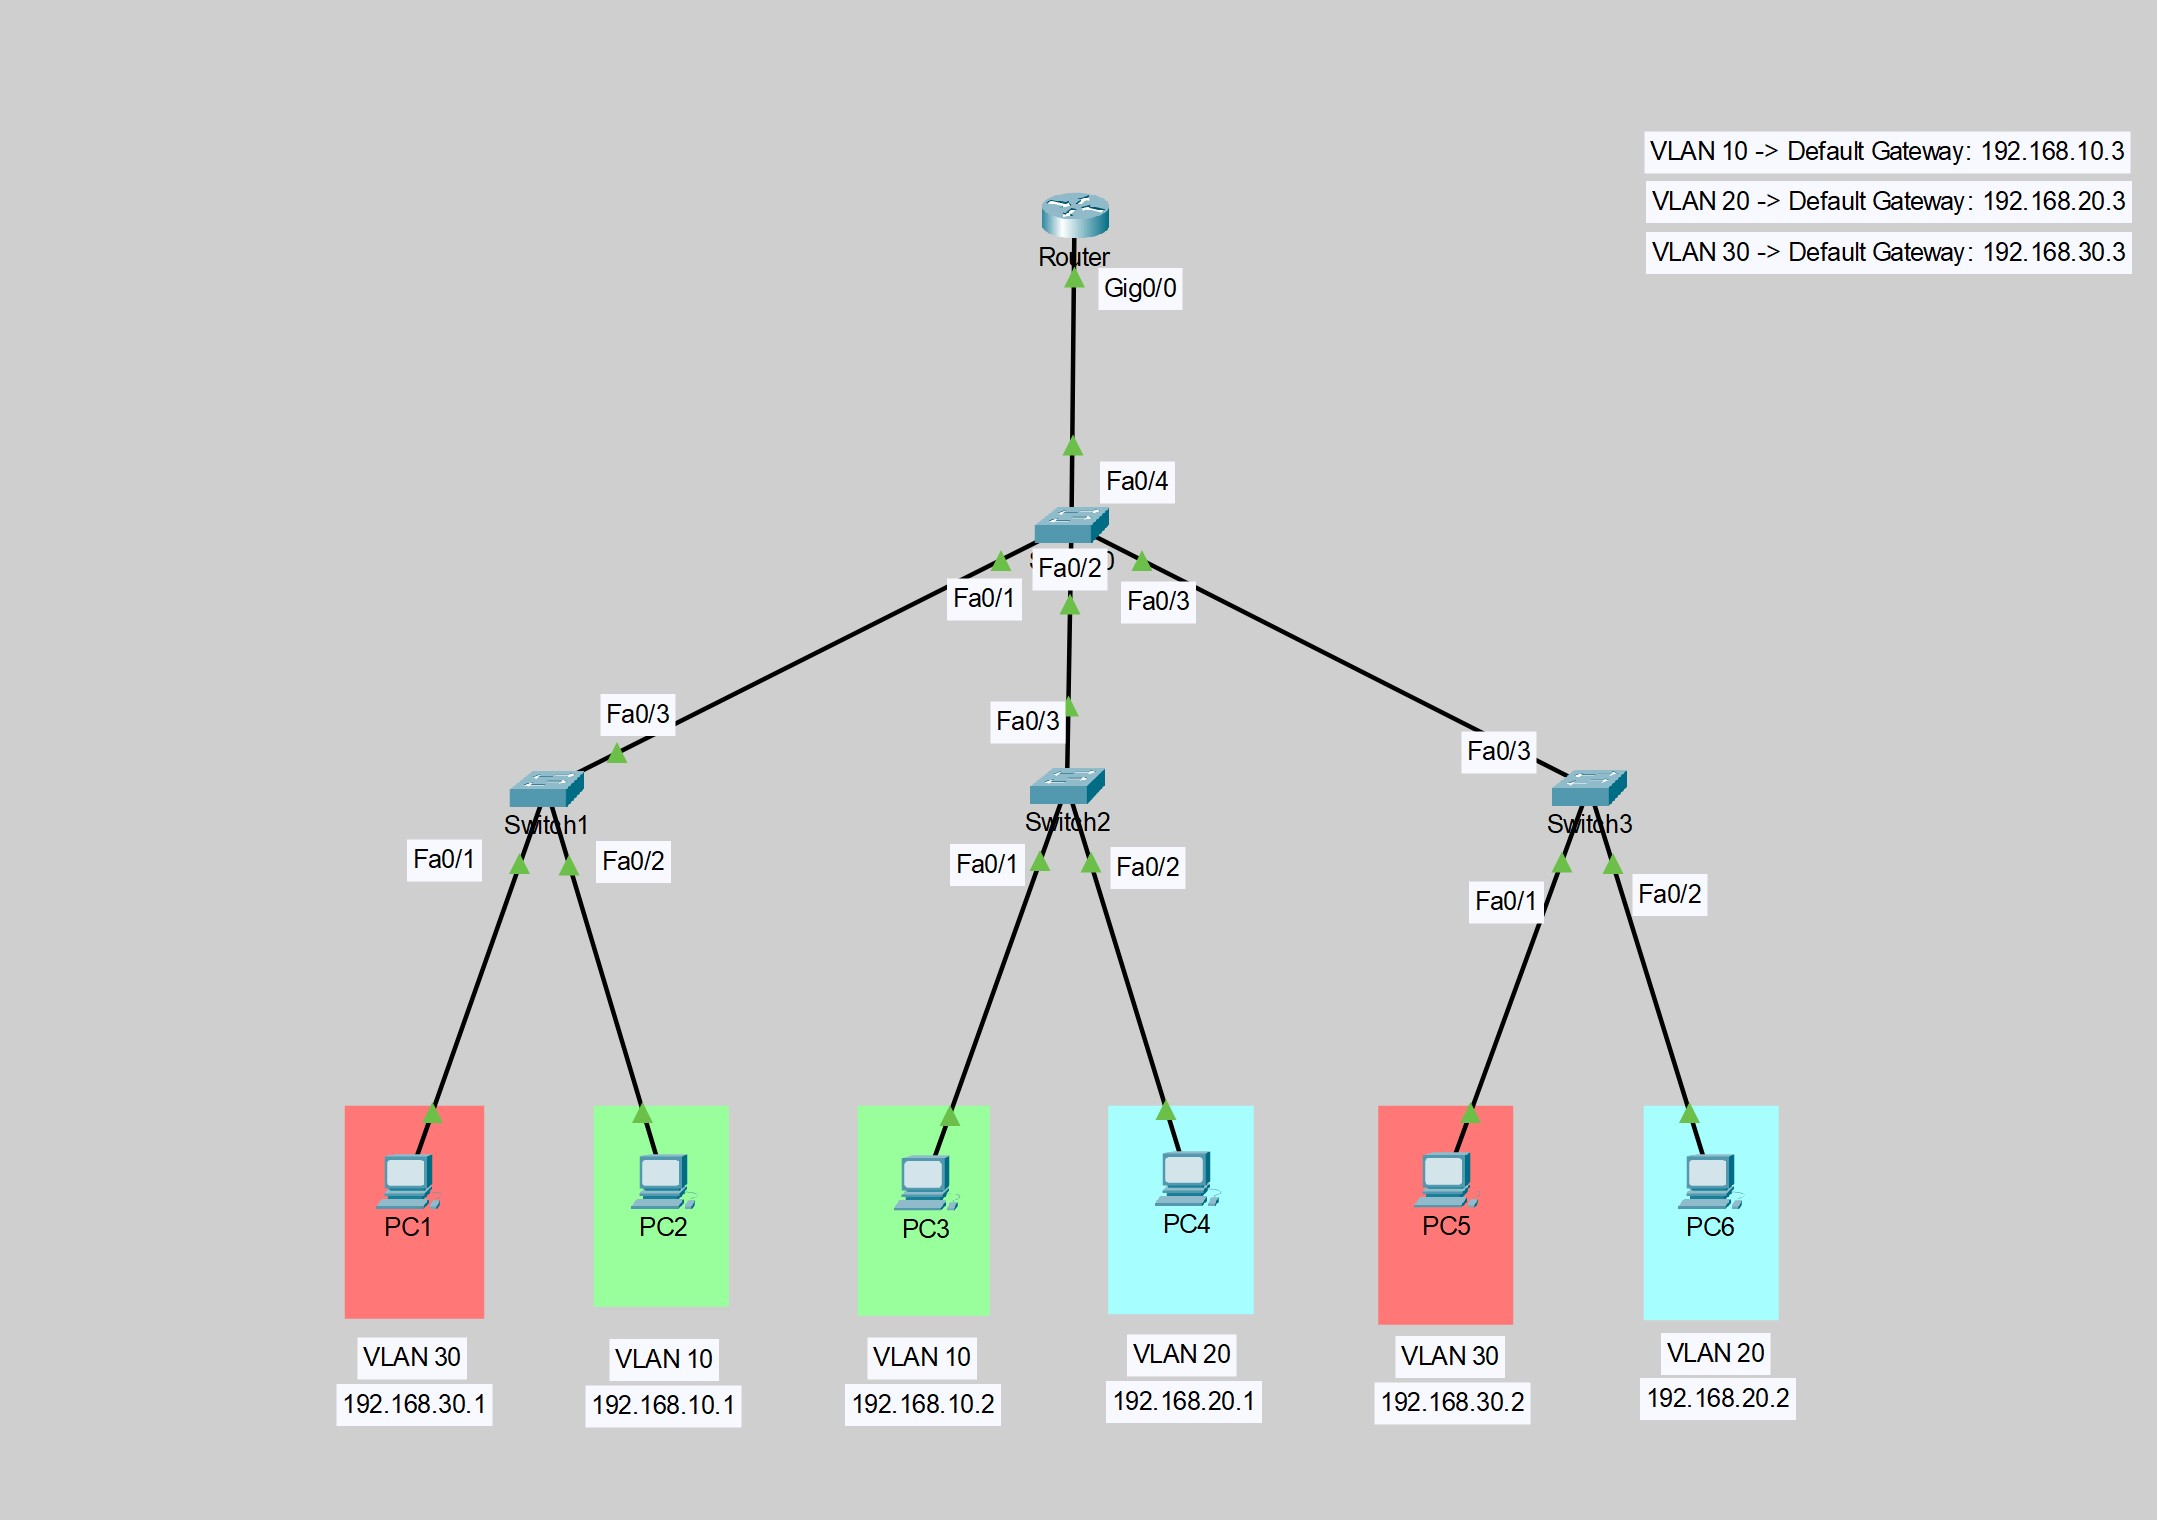
\includegraphics[width=0.9\textwidth]{ROAS.jpg}
    \caption{\textit{Network topology created using the Packet Tracer Simulator.}}

    \label{fig:packet_tracer_topology}
\end{figure}
\vspace{1cm}

\section{Scenario}
\begin{itemize}
    \item \textbf{A router} is connected to three \textbf{Layer 2 switches} using a \textbf{trunk link}.
    \item Each PC is assigned to a specific \textbf{VLAN (10, 20, or 30)}.
    \item The \textbf{router performs inter-VLAN routing} using \textbf{subinterfaces}.
    \item Each VLAN has a corresponding \textbf{default gateway} assigned on the router.
\end{itemize}



\chapter{Router-on-a-Stick (ROAS)}

\begin{enumerate}
    \item Configure the \texttt{GigabitEthernet0/0} interface as a trunk.
    \item Assign subinterface \texttt{0/0.10} for VLAN 10 with IP \texttt{192.168.10.1/24}.
    \item Assign subinterface \texttt{0/0.20} for VLAN 20 with IP \texttt{192.168.20.1/24}.
    \item Assign subinterface \texttt{0/0.30} for VLAN 30 with IP \texttt{192.168.30.1/24}.
    \item Configure \texttt{FastEthernet0/1} as a trunk on Switch1.
    \item Configure \texttt{FastEthernet0/1} as a trunk on Switch2.
    \item Configure \texttt{FastEthernet0/1} as a trunk on Switch3.
    \item Assign \texttt{FastEthernet0/2} on Switch1 to VLAN 10.
    \item Assign \texttt{FastEthernet0/2} on Switch2 to VLAN 20.
    \item Assign \texttt{FastEthernet0/2} on Switch3 to VLAN 30.
    \item Verify trunking status on switches.
    \item Show the current VLAN configuration.
    \item Display the routing table to check inter-VLAN routing.
    \item Show all subinterfaces configured on the router.
    \item Check encapsulation settings for all subinterfaces.
    \item Verify if PC1 can ping PC2.
    \item Verify if PC3 can ping PC1.
    \item Save the running configuration.
    \item Debug IP routing issues.
    \item Remove subinterface \texttt{0/0.30}.
    \item Disable the trunk link on Switch1.
    \item Reset the router configuration.
\end{enumerate}

\newpage

\chapter{Network Topology for Multilayer Switch (MLS)}

\section{Network Topology}
The topology below shows a \textbf{Multilayer Switch (MLS) network} where multiple VLANs are implemented. The goal of this workbook is to configure the \textbf{Layer 3 switch} for inter-VLAN routing and ensure successful communication between VLANs.


\begin{figure}[h]
    \centering
    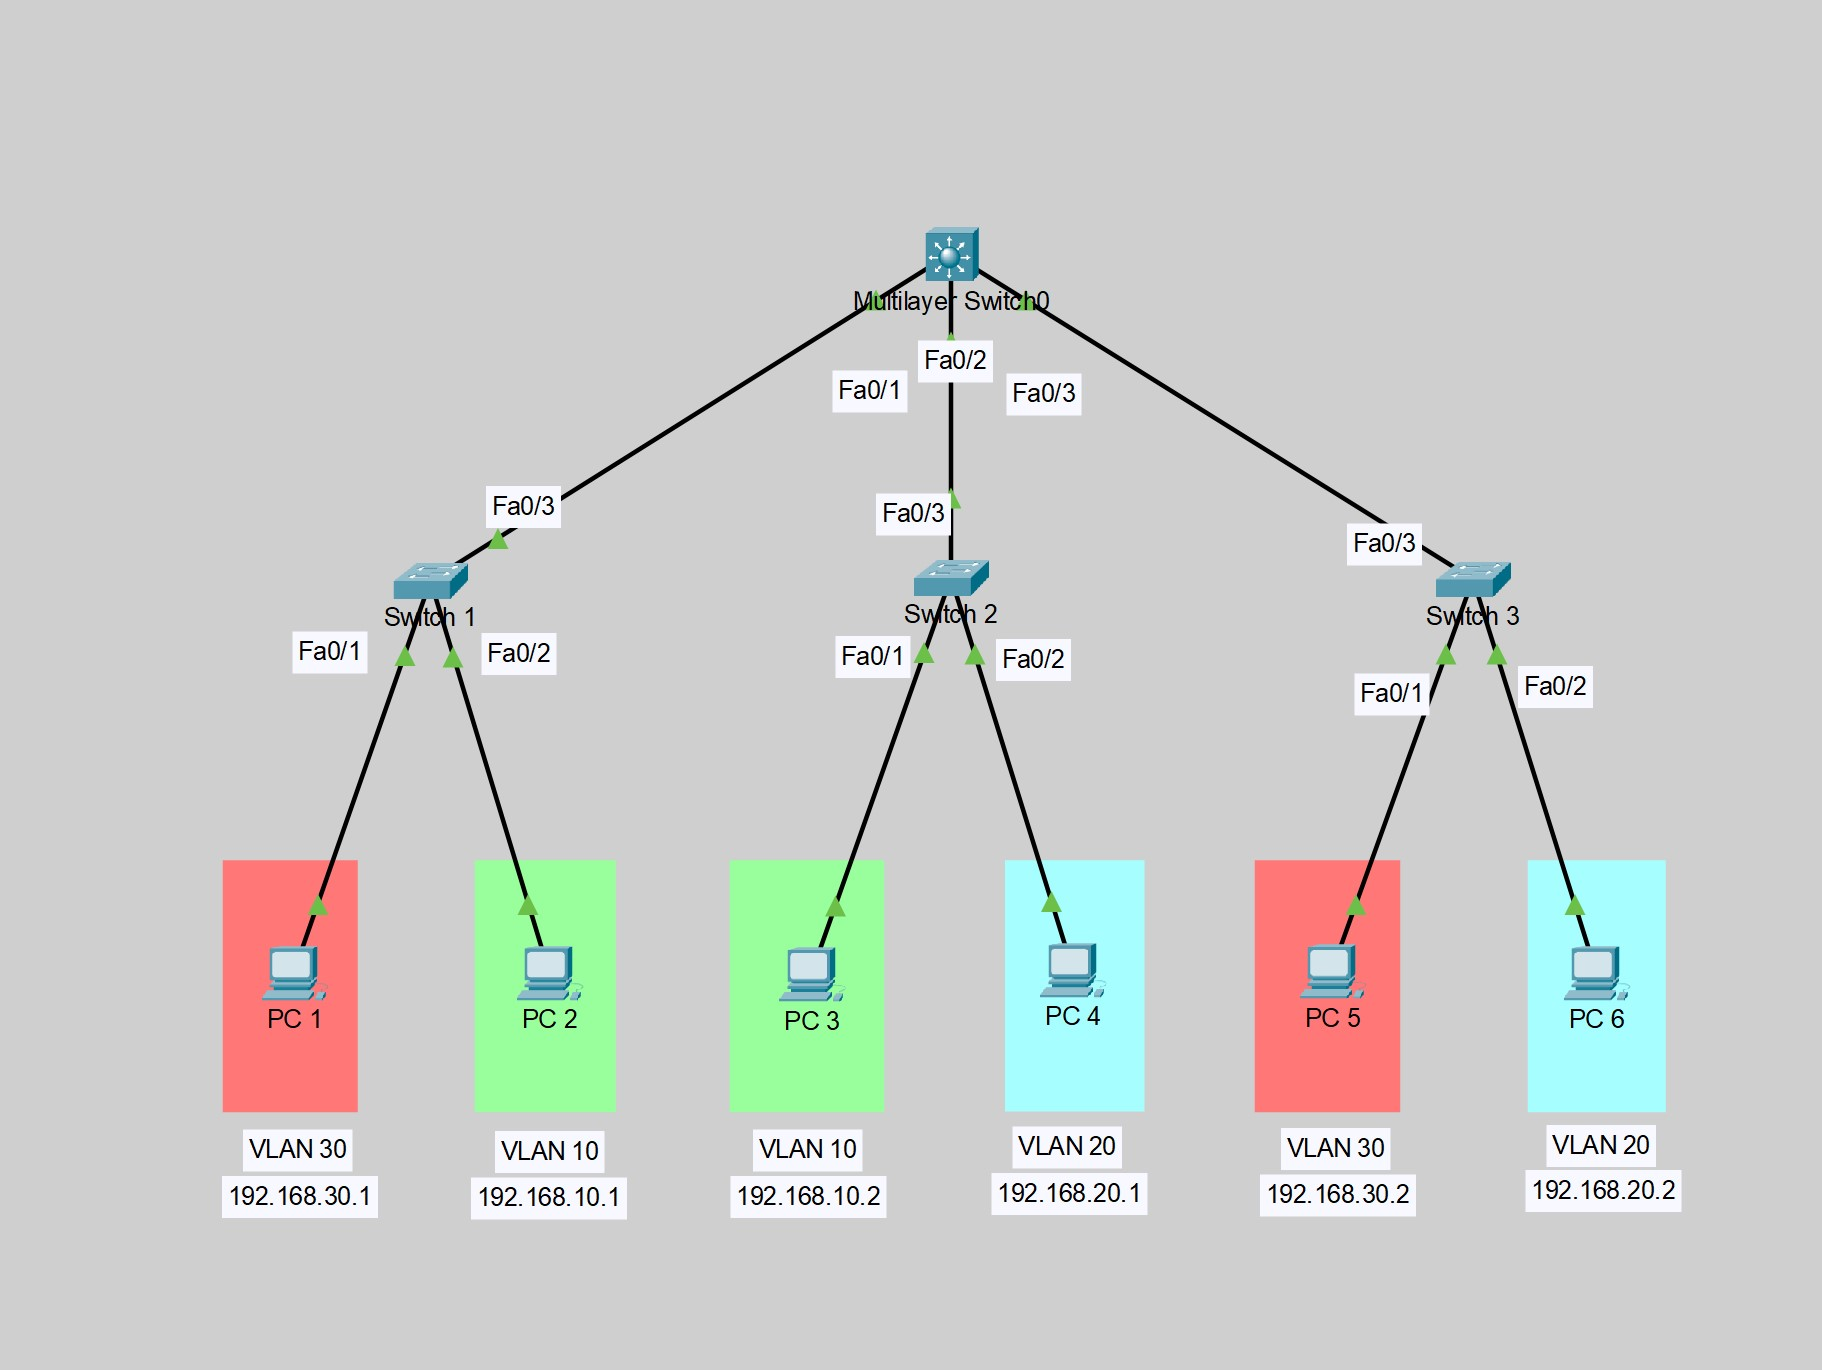
\includegraphics[width=0.9\textwidth]{MLS.jpg}
    \caption{\textit{Network topology created using the Packet Tracer Simulator.}}

    \label{fig:packet_tracer_topology}
\end{figure}


\section{Scenario}
\begin{itemize}
    \item This network consists of \textbf{three access switches}, \textbf{one multilayer switch}, and \textbf{six PCs}.
    \item Each PC is assigned to a specific \textbf{VLAN (10, 20, or 30)}.
    \item The \textbf{multilayer switch} will perform \textbf{inter-VLAN routing} using \textbf{SVI (Switched Virtual Interfaces)}.
\end{itemize}

\chapter{Multilayer Switch (MLS)}

\begin{enumerate}
    \item Create VLAN 10, 20, and 30 on a multilayer switch
    \item Set interface range \texttt{FastEthernet0/1 - 0/2} as trunk ports on multilayer switch.
    \item Verify VLAN configurations on the multilayer switch.
    \item Show the trunking status of all interfaces on multilayer switch.
    \item Set the \texttt{Fa0/3} link on switches 1, 2, and 3 to trunk mode.
    \item Set the \texttt{Fa0/1} link on Switch 1 to connect PC1 in VLAN 30 and the \texttt{Fa0/2} link to connect PC2 in VLAN 10.
    \item Set the \texttt{Fa0/1} link on Switch 2 to connect PC3 in VLAN 10 and the \texttt{Fa0/2} link to connect PC4 in VLAN 20.
    \item Set the \texttt{Fa0/1} link on Switch 3 to connect PC5 in VLAN 30 and the \texttt{Fa0/2} link to connect PC6 in VLAN 20.
    \item Configure the gateway addresses on the multilayer switch (SVI interfaces for VLANs).
    \item Perform an inter-VLAN connectivity test using the ping command.

    
\end{enumerate}

\part{Answer Key and Explanations}


\chapter{Router-on-a-Stick (ROAS) - Answers}

\begin{enumerate}
\item{Configure the \texttt{GigabitEthernet0/0} interface as a trunk}

\begin{lstlisting}
Router(config)# interface GigabitEthernet0/0
Router(config-if)# no shutdown
Router(config-if)# exit
\end{lstlisting}

\item{Assign subinterface \texttt{0/0.10} for VLAN 10 with IP \texttt{192.168.10.1/24}}

\begin{lstlisting}
Router(config)# interface GigabitEthernet0/0.10
Router(config-subif)# encapsulation dot1Q 10
Router(config-subif)# ip address 192.168.10.1 255.255.255.0
Router(config-subif)# exit
\end{lstlisting}

\item{Assign subinterface \texttt{0/0.20} for VLAN 20 with IP \texttt{192.168.20.1/24}}

\begin{lstlisting}
Router(config)# interface GigabitEthernet0/0.20
Router(config-subif)# encapsulation dot1Q 20
Router(config-subif)# ip address 192.168.20.1 255.255.255.0
Router(config-subif)# exit
\end{lstlisting}

\item{Assign subinterface \texttt{0/0.30} for VLAN 30 with IP \texttt{192.168.30.1/24}}

\begin{lstlisting}
Router(config)# interface GigabitEthernet0/0.30
Router(config-subif)# encapsulation dot1Q 30
Router(config-subif)# ip address 192.168.30.1 255.255.255.0
Router(config-subif)# exit
\end{lstlisting}



\item{Configure \texttt{FastEthernet0/1} as a trunk on Switch1.}

\begin{lstlisting}
Switch1(config)# interface FastEthernet0/1
Switch1(config-if)# switchport mode trunk
Switch1(config-if)# exit
\end{lstlisting}

\item{Configure \texttt{FastEthernet0/1} as a trunk on Switch2.}
\begin{lstlisting}
Switch2(config)# interface FastEthernet0/1
Switch2(config-if)# switchport mode trunk
Switch2(config-if)# exit
\end{lstlisting}

\item{Configure \texttt{FastEthernet0/1} as a trunk on Switch3.}
\begin{lstlisting}
Switch3(config)# interface FastEthernet0/1
Switch3(config-if)# switchport mode trunk
Switch3(config-if)# exit
\end{lstlisting}

\item{Assign \texttt{FastEthernet0/2} on Switch1 to VLAN 10}

\begin{lstlisting}
Switch1(config)# interface FastEthernet0/2
Switch1(config-if)# switchport mode access
Switch1(config-if)# switchport access vlan 10
Switch1(config-if)# exit
\end{lstlisting}

\item{Assign \texttt{FastEthernet0/2} on Switch2 to VLAN 20}

\begin{lstlisting}
Switch2(config)# interface FastEthernet0/2
Switch2(config-if)# switchport mode access
Switch2(config-if)# switchport access vlan 20
Switch2(config-if)# exit
\end{lstlisting}

\item{Assign \texttt{FastEthernet0/2} on Switch3 to VLAN 30}
\begin{lstlisting}

Switch3(config)# interface FastEthernet0/2
Switch3(config-if)# switchport mode access
Switch3(config-if)# switchport access vlan 30
Switch3(config-if)# exit
\end{lstlisting}


\item{Verify \texttt{trunking status} on switches.}

\begin{lstlisting}
Switch# show interfaces trunk
\end{lstlisting}

\item{Show current VLAN configuration}

\begin{lstlisting}
Switch# show vlan brief
\end{lstlisting}

\item{Display the routing table}

\begin{lstlisting}
Router# show ip route
\end{lstlisting}

\item{Show all subinterfaces}

\begin{lstlisting}
Router# show ip interface brief
\end{lstlisting}

\item{Check encapsulation settings}

\begin{lstlisting}
Router# show interfaces GigabitEthernet0/0.10
Router# show interfaces GigabitEthernet0/0.20
Router# show interfaces GigabitEthernet0/0.30
\end{lstlisting}

\item{Verify if PC1 can ping PC2.}
\item{Verify if PC3 can ping PC1.}
 
\begin{lstlisting}
PC1> ping 192.168.20.1
PC3> ping 192.168.10.1
\end{lstlisting}

\item{Save the running configuration}

\begin{lstlisting}
Router# write memory
Switch# write memory
\end{lstlisting}

\item{Debug IP routing issues}

\begin{lstlisting}
Router# debug ip routing
\end{lstlisting}

\item{Remove subinterface 0/0.30}

\begin{lstlisting}
Router(config)# no interface GigabitEthernet0/0.30
\end{lstlisting}

\item{Disable trunk link on Switch1}

\begin{lstlisting}
Switch1(config)# interface FastEthernet0/1
Switch1(config-if)# switchport mode access
Switch1(config-if)# exit
\end{lstlisting}

\item{Reset the router configuration}

\begin{lstlisting}
Router# write erase
Router# reload
\end{lstlisting}

\end{enumerate}

\newpage

\chapter{Multilayer Switch (MLS) - Answers}

\begin{enumerate}
    \item Create VLAN 10, 20, and 30 on a multilayer switch.
    \begin{lstlisting}
    configure terminal
    vlan 10
    vlan 20
    vlan 30
    exit
    \end{lstlisting}

    \item Set interface range \texttt{FastEthernet0/1 - 0/2} as trunk ports on multilayer switch.
    \begin{lstlisting}
    configure terminal
    interface range FastEthernet0/1 - 2
    switchport mode trunk
    exit
    \end{lstlisting}
    \item Verify VLAN configurations on the multilayer switch.
    \begin{lstlisting}
    show vlan brief
    \end{lstlisting}

    \item Show the trunking status of all interfaces on multilayer switch.
    \begin{lstlisting}
    show interfaces trunk
    \end{lstlisting}
    \item Set the \texttt{Fa0/3} link on switches 1, 2, and 3 to trunk mode.
    For Switch 1:
    \begin{lstlisting}
    configure terminal
    interface FastEthernet0/3
    switchport mode trunk
    exit
    \end{lstlisting}

    For Switch 2:
    \begin{lstlisting}
    configure terminal
    interface FastEthernet0/3
    switchport mode trunk
    exit
    \end{lstlisting}

    For Switch 3:
    \begin{lstlisting}
    configure terminal
    interface FastEthernet0/3
    switchport mode trunk
    exit
    \end{lstlisting}
    \item Set the \texttt{Fa0/1} link on Switch 1 to connect PC1 in VLAN 30 and the \texttt{Fa0/2} link to connect PC2 in VLAN 10.
    \begin{lstlisting}
    configure terminal
    interface FastEthernet0/1
    switchport mode access
    switchport access vlan 30
    exit
    
    interface FastEthernet0/2
    switchport mode access
    switchport access vlan 10
    exit
    \end{lstlisting}
    \item Set the \texttt{Fa0/1} link on Switch 2 to connect PC3 in VLAN 10 and the \texttt{Fa0/2} link to connect PC4 in VLAN 20.
    \begin{lstlisting}
    configure terminal
    interface FastEthernet0/1
    switchport mode access
    switchport access vlan 10
    exit

    interface FastEthernet0/2
    switchport mode access
    switchport access vlan 20
    exit
    \end{lstlisting}
    \item Set the \texttt{Fa0/1} link on Switch 3 to connect PC5 in VLAN 30 and the \texttt{Fa0/2} link to connect PC6 in VLAN 20.
    \begin{lstlisting}
    configure terminal
    interface FastEthernet0/1
    switchport mode access
    switchport access vlan 30
    exit
        
    interface FastEthernet0/2
    switchport mode access
    switchport access vlan 20
    exit
    \end{lstlisting}
    \item Configure the gateway addresses on the multilayer switch (SVI interfaces for VLANs).
    \begin{lstlisting}
    configure terminal
    interface Vlan10
    ip address 192.168.10.3 255.255.255.0
    no shutdown
    exit
        
    interface Vlan20
    ip address 192.168.20.3 255.255.255.0
    no shutdown
    exit
        
    interface Vlan30
    ip address 192.168.30.3 255.255.255.0
    no shutdown
    exit
    \end{lstlisting}
    \item Perform an inter-VLAN connectivity test using the ping command.
    
    \textit{Step 1: Verify VLAN Interface Status}
    \newline
    \newline
    First, check if the VLAN interfaces (SVIs) are active:
    \begin{lstlisting}
    show ip interface brief
    \end{lstlisting}
    Ensure that the VLAN interfaces (\texttt{Vlan10, Vlan20, Vlan30}) have assigned IP addresses and are \textbf{up}.
    
    \textit{Step 2: Ping Between VLANs}
    \newline
    \newline
    Run the following ping tests from the Multilayer Switch:
    
    Ping from VLAN 10 (\texttt{192.168.10.3}) to VLAN 20 (\texttt{192.168.20.3})
    \begin{lstlisting}
    ping 192.168.20.3
    \end{lstlisting}
    
    Ping from VLAN 10 (\texttt{192.168.10.3}) to VLAN 30 (\texttt{192.168.30.3})
    \begin{lstlisting}
    ping 192.168.30.3
    \end{lstlisting}
    
    Ping from VLAN 20 (\texttt{192.168.20.3}) to VLAN 30 (\texttt{192.168.30.3})
    \begin{lstlisting}
    ping 192.168.30.3
    \end{lstlisting}
    
    \textit{Step 3: Ping from a PC}
    \newline
    \newline
    From \textbf{PC1 (VLAN 30, IP: 192.168.30.10)}, test connectivity to \textbf{PC2 (VLAN 10, IP: 192.168.10.10)}:
    \begin{lstlisting}
    ping 192.168.10.10
    \end{lstlisting}
    
    From \textbf{PC4 (VLAN 20, IP: 192.168.20.10)}, test connectivity to \textbf{PC5 (VLAN 30, IP: 192.168.30.10)}:
    \begin{lstlisting}
    ping 192.168.30.10
    \end{lstlisting}
    
    \section*{Expected Output}
    If inter-VLAN routing is \textbf{correctly configured}, the \texttt{ping} should be successful. If there is an issue, check:
    \begin{itemize}
        \item \textbf{SVI configurations} (\texttt{show run})
        \item \textbf{Routing status} (\texttt{show ip route})
        \item \textbf{Trunk links between switches} (\texttt{show interfaces trunk})
    \end{itemize}
    
    \textbf{\checkmark This confirms that inter-VLAN communication is working properly!}
    


\end{enumerate}

\end{document}
